\section{Analog Signal Chain}
\begin{minipage}{11cm}
	Embeddes Systems interact with the the Outer Real World. In this Environment, many Signals in the outer Real World are Analog. Analog Signals must be transferred into their Digital Representation to be processed. 
\end{minipage}
\begin{minipage}{6cm}
	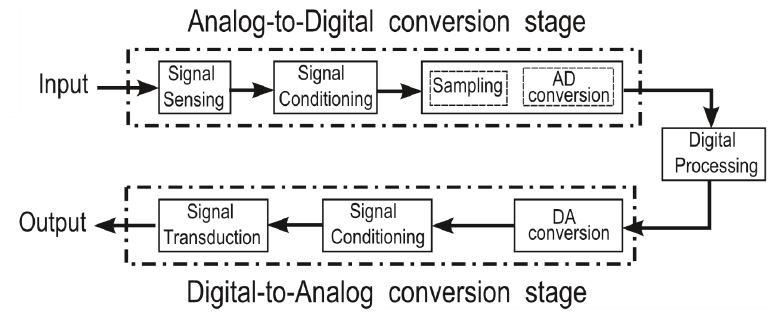
\includegraphics[width=8cm]{images/signalchain.jpg}
\end{minipage}
\subsection{Mixed-Signal Processing Chain}
\begin{itemize}
	\item Signal Chain
	\subitem refers to a series of Signal-Conditioning Electronic Components connected to each other
	\item Signal Sensing
	\subitem Active and Passive Sensors, Sensor Characteristics
	\item Signal Conditioning
	\subitem Amplification,Linearizing, Filtering
	\item Signal Transduction
	\subitem Active and Passive Sensors, Sensor Characteristics
\end{itemize}
\subsection{Comparator, ADC, DAC}
\subsubsection{Comparator}
\begin{minipage}{12cm}
	\begin{itemize}
		\item Compare voltage with reference voltage level
		\item if Input Voltage higher than reference $\rightarrow$ Mark
		\item If Input Voltage lower than reference $\rightarrow$ Space
		\item Hysterese alos possible
	\end{itemize}
\end{minipage}
\begin{minipage}{4cm}
	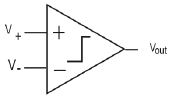
\includegraphics[width=4cm]{images/comparator.jpg}
\end{minipage}
\begin{multicols}{2}
\subsubsection{ADC}
\begin{itemize}
	\item Analog-Digital-Converter
	\item From Voltage to Digital Value (Bits)
	\item Voltage ist quantizied and samplet
\end{itemize}
\subsubsection{DAC}
\begin{itemize}
	\item Digital-Analog-Converter
	\item From Digital Value to Voltage
	\item From Bit to voltage 
\end{itemize}
\subsubsection{Nyquist Principle}
\begin{itemize}
	\item The Sampling Frequence must  be at east double of the highest frequency
	\item $f_s \ge 2 \cdot f_h$
\end{itemize}
\subsubsection{Aliasing}
\begin{itemize}
	\item when a signal with frequency is samplet with $f_s$ than the same Samples will apply to another Signal with Frequency of $k \cdot f_s \pm f$
	\item use Low-Pass or Band-Pass Antialiasing Filters to solve
\end{itemize}
\subsubsection{Quantization}
\begin{itemize}
	\item Full Scale Range $VFS=V_{max}-V_{min}$
	\item Quantization Error $ \frac{1}{2} \Delta$
	\item Resolution $\Delta = \frac{V_{max}-V_{min}}{2^n}$
\end{itemize}
\subsubsection{MSP430 ADC \& DAC Infrastructure}
\begin{itemize}
	\item 8 Analog Comparators
	\item 8 or 12-Bit DAC
	\item SAR, Sigma-Delta ADC with variety Resolution
	\end{itemize}
\end{multicols}
\clearpage
